%%
%% This is file `sample-authordraft.tex',
%% generated with the docstrip utility.
%%
%% The original source files were:
%%
%% samples.dtx  (with options: `authordraft')
%% 
%% IMPORTANT NOTICE:
%% 
%% For the copyright see the source file.
%% 
%% Any modified versions of this file must be renamed
%% with new filenames distinct from sample-authordraft.tex.
%% 
%% For distribution of the original source see the terms
%% for copying and modification in the file samples.dtx.
%% 
%% This generated file may be distributed as long as the
%% original source files, as listed above, are part of the
%% same distribution. (The sources need not necessarily be
%% in the same archive or directory.)
%%
%% Commands for TeXCount
%TC:macro \cite [option:text,text]
%TC:macro \citep [option:text,text]
%TC:macro \citet [option:text,text]
%TC:envir table 0 1
%TC:envir table* 0 1
%TC:envir tabular [ignore] word
%TC:envir displaymath 0 word
%TC:envir math 0 word
%TC:envir comment 0 0
%%
%%
%% The first command in your LaTeX source must be the \documentclass command.
%% \documentclass[sigconf,authordraft]{acmart}
\documentclass[sigconf,authorversion,nonacm]{acmart}
\usepackage{graphicx}
\usepackage{multirow}
\graphicspath{ {./images/} }
%% NOTE that a single column version may required for 
%% submission and peer review. This can be done by changing
%% the \doucmentclass[...]{acmart} in this template to 
%% \documentclass[manuscript,screen]{acmart}
%% 
%% To ensure 100% compatibility, please check the white list of
%% approved LaTeX packages to be used with the Master Article Template at
%% https://www.acm.org/publications/taps/whitelist-of-latex-packages 
%% before creating your document. The white list page provides 
%% information on how to submit additional LaTeX packages for 
%% review and adoption.
%% Fonts used in the template cannot be substituted; margin 
%% adjustments are not allowed.

%%
%% \BibTeX command to typeset BibTeX logo in the docs
\AtBeginDocument{%
  \providecommand\BibTeX{{%
    \normalfont B\kern-0.5em{\scshape i\kern-0.25em b}\kern-0.8em\TeX}}}

%% Rights management information.  This information is sent to you
%% when you complete the rights form.  These commands have SAMPLE
%% values in them; it is your responsibility as an author to replace
%% the commands and values with those provided to you when you
%% complete the rights form.
% \setcopyright{acmcopyright}
% \copyrightyear{2018}
% \acmYear{2018}
% \acmDOI{XXXXXXX.XXXXXXX}

%% These commands are for a PROCEEDINGS abstract or paper.
% \acmConference[Conference acronym 'XX]{Make sure to enter the correct
%   conference title from your rights confirmation emai}{June 03--05,
%   2018}{Woodstock, NY}
%
%  Uncomment \acmBooktitle if th title of the proceedings is different
%  from ``Proceedings of ...''!
%
%\acmBooktitle{Woodstock '18: ACM Symposium on Neural Gaze Detection,
%  June 03--05, 2018, Woodstock, NY} 
% \acmPrice{15.00}
% \acmISBN{978-1-4503-XXXX-X/18/06}


%%
%% Submission ID.
%% Use this when submitting an article to a sponsored event. You'll
%% receive a unique submission ID from the organizers
%% of the event, and this ID should be used as the parameter to this command.
%%\acmSubmissionID{123-A56-BU3}

%%
%% For managing citations, it is recommended to use bibliography
%% files in BibTeX format.
%%
%% You can then either use BibTeX with the ACM-Reference-Format style,
%% or BibLaTeX with the acmnumeric or acmauthoryear sytles, that include
%% support for advanced citation of software artefact from the
%% biblatex-software package, also separately available on CTAN.
%%
%% Look at the sample-*-biblatex.tex files for templates showcasing
%% the biblatex styles.
%%

%%
%% For managing citations, it is recommended to use bibliography
%% files in BibTeX format.
%%
%% You can then either use BibTeX with the ACM-Reference-Format style,
%% or BibLaTeX with the acmnumeric or acmauthoryear sytles, that include
%% support for advanced citation of software artefact from the
%% biblatex-software package, also separately available on CTAN.
%%
%% Look at the sample-*-biblatex.tex files for templates showcasing
%% the biblatex styles.
%%

%%
%% The majority of ACM publications use numbered citations and
%% references.  The command \citestyle{authoryear} switches to the
%% "author year" style.
%%
%% If you are preparing content for an event
%% sponsored by ACM SIGGRAPH, you must use the "author year" style of
%% citations and references.
%% Uncommenting
%% the next command will enable that style.
%%\citestyle{acmauthoryear}

%%
%% end of the preamble, start of the body of the document source.
\begin{document}

%%
%% The "title" command has an optional parameter,
%% allowing the author to define a "short title" to be used in page headers.
\title{Metacodenition: A Tool to Scaffold the Problem-Solving Process for Novice Programmers}

%%
%% The "author" command and its associated commands are used to define
%% the authors and their affiliations.
%% Of note is the shared affiliation of the first two authors, and the
%% "authornote" and "authornotemark" commands
%% used to denote shared contribution to the research.
\author{Yulia Pechorina}
\affiliation{%
  \institution{The University of Auckland}
  \streetaddress{20 Symonds Street}
  \city{Auckland}
  \country{New Zealand}}
\email{ypec413@auckland.ac.nz}
%%
%% By default, the full list of authors will be used in the page
%% headers. Often, this list is too long, and will overlap
%% other information printed in the page headers. This command allows
%% the author to define a more concise list
%% of authors' names for this purpose.
\renewcommand{\shortauthors}{Yulia Pechorina}

%%
%% The abstract is a short summary of the work to be presented in the
%% article.
\begin{abstract}
Problem-solving is a crucial skill for programmers, but one that novices can find challenging to develop. Despite the importance of problem-solving skills and the many frameworks which exist to formalise them, most introductory programming courses do not explicitly teach them. Programming educators find it challenging to teach problem-solving, as students must develop metacognitive awareness, that is, an awareness of one's thinking, to identify their problem-solving state. We contribute a tool called Metacodenition, which provides metacognitive scaffolding for an existing problem-solving framework. Our evaluation shows that Metacodenition's scaffolding improves performance on code-writing tasks and students view Metacodenition to be a helpful tool they would use again voluntarily.
\end{abstract}

%%
%% The code below is generated by the tool at http://dl.acm.org/ccs.cfm.
%% Please copy and paste the code instead of the example below.
%%
\begin{CCSXML}
<ccs2012>
   <concept>
       <concept_id>10003456.10003457.10003527</concept_id>
       <concept_desc>Social and professional topics~Computing education</concept_desc>
       <concept_significance>500</concept_significance>
   </concept>
 </ccs2012>
\end{CCSXML}

\ccsdesc[500]{Social and professional topics~Computing education}

%%
%% Keywords. The author(s) should pick words that accurately describe
%% the work being presented. Separate the keywords with commas.
\keywords{metacognition, problem-solving, software engineering education}

% \received{20 February 2007}
% \received[revised]{12 March 2009}
% \received[accepted]{5 June 2009}

%%
%% This command processes the author and affiliation and title
%% information and builds the first part of the formatted document.
\maketitle

\section{Introduction}
Learning to program requires students to develop several skills, one of which is problem-solving \cite{lakanen2015, bruce2003}. It is widely accepted that problem-solving is both a critical skill \cite{gomes2007}, and one of the most difficult skills for novices to develop \cite{medeiros2019}. Further, an ITiCSE working group study found that many students in introductory programming courses lacked problem-solving skills \cite{lister2004}.

Poor problem-solving skills often persist throughout a student's degree. A study by Radermacher et al. investigating the skill gap between software engineering graduates and industry expectations found that a lack of problem-solving skills is one of the two most common issues which prevents graduate software engineers from being employed \cite{radermacher2014}. The authors also found that employers placed the importance of non-technical skills, such as problem-solving skills, above technical skills. Some employers were willing to hire graduates who lacked technical ability so long as they demonstrated good problem-solving skills.

A factor for poor problem-solving skills in novices is the curriculum of introductory programming courses. Programming skills taught in introductory programming courses can be divided into programming knowledge and programming problem-solving strategies. Programming knowledge refers to the syntax and semantics of programming, whereas programming problem-solving strategies refer to how one applies programming knowledge to solve a problem \cite{deraat2009}. In a typical course curriculum, programming knowledge is explicitly taught, whereas problem-solving strategies are often implicitly taught \cite{muller2007}.

Even when problem-solving strategies are explicitly taught, novice programmers often face difficulty learning problem-solving because they lack metacognitive awareness \cite{anneli1993, loksa2016, mani2013}. Metacognitive awareness means being aware of one's own thinking and problem-solving strategies \cite{gibson1996}, and plays a significant role in programming \cite{parham2010}. When programming, students use metacognition to move between the steps of problem-solving process and decide when to revisit steps \cite{parham2010}.

Loksa et al. developed a problem-solving framework, along with interventions for this framework, to promote metacognitive awareness \cite{loksa20162}. Multiple studies exist that build on Loksa et al.'s framework and propose other interventions to promote metacognition further. However, current work is generally limited to interventions for a single stage of a problem-solving framework at a time. These interventions individually are effective at teaching students how to problem solve, increasing their metacognitive awareness and performance in their courses. To our knowledge, only one tool, TextCode \cite{corno2021}, has been developed to cater to multiple problem-solving stages. However, TextCode does not scaffold the entire problem-solving process; it only scaffolds the process up to the implementing a solution stage; the evaluation stage is missed. The evaluation stage is included in the majority of problem-solving frameworks and is crucial for ensuring the solution meets the problem requirements and making any necessary modifications to the solution.

In this work, we investigate whether combining multiple problem-solving stages into a tool will make it more effective for teaching problem-solving than a tool that only integrates one, by developing a tool that caters to multiple stages Loksa et al.'s framework at once.

Our contribution is an integrated development environment (IDE) called Metacodenition, designed to provide metacognitive scaffolding during code writing exercises. We outline the design of Metacodenition and then evaluate its effectiveness through a study involving 821 first-year engineering students taking an introductory programming course. We investigate the following research questions:
\begin{itemize}
\item RQ1: What are students' perceptions toward using Metacodenition for problem-solving activities?
\item RQ2: Does the scaffolding provided by Metacodenition improve performance on code-writing tasks?
\end{itemize}

The remainder of this paper is organized as follows. Section 2 reviews related work on strategies, frameworks, and interventions designed to aid novices in developing problem-solving skills. In Section 3, we present our approach to designing Metacodenition. We then cover our process in evaluating Metacodenition in Section 4 and report the results and discussion of this evaluation in Sections 5. Finally, we conclude in Section 6.

\section{Related Work}

\subsection{Problem-solving frameworks}
Loksa et al. \cite{loksa20162} developed a programming-specific problem-solving framework consisting of the following stages: (1) reinterpreting the problem prompt, (2) searching for analogous problems, (3) searching for solutions, (4) evaluating a potential solution, (5) implementing a solution, and (6) evaluating an implemented solution (see Table \ref{tab:loksaFramework}). 

\begin{table}
  \caption{Loksa et al.'s problem-solving stages}
  \label{tab:loksaFramework}
  \begin{tabular}{c|p{35mm}|p{35mm}}
    \toprule
    \#&Stage&Description\\
    \midrule
    1&Reinterpreting the problem prompt&Understanding and interpreting the problem statement and requirements\\
    \midrule
    2&Searching for analogous problems&Drawing upon previously encountered problems \\
    \midrule
    3&Searching for solutions&Seeking solutions that will solve the problem\\
    \midrule
    4&Evaluating a potential solution&Evaluating whether the solution meets problem requirements, often using prototyping techniques such as pseudo code\\
    \midrule
    5&Implementing a solution&Writing the solution code \\
    \midrule
    6&Evaluating an implemented solution&Evaluating whether the current solution meets the problem requirements, usually through testing and debugging\\
    \bottomrule
  \end{tabular}
\end{table}

A controlled experiment with 48 students was conducted to measure the effect of teaching Loksa et al.’s framework along with interventions to motivate students to think about their progress along the stages of the problem-solving framework. The experimental and control groups participated in separate coding camps, and the experimental group had multiple interventions in their camp schedule. Intervention (1) was a 1-hour problem-solving lecture. Intervention (2) was a prompt when a student requested help from an instructor, asking them to identify their current problem-solving stage. Intervention (3) was a physical handout of the problem-solving stages. Intervention (4) was hints categorized under the problem-solving stages added to the student’s IDE. They found that students in the experimental group had more detailed explanations of their problem-solving strategies, required help with design and selection rather than debugging, relied less on the instructors, and had greater productivity and scores. While these interventions were successful, they can be difficult to implement at scale due to no automation for interventions 1 to 3. Intervention 2 had especially low scalability, as it required 1:1 contact between the instructor and student. 

A framework with a greater focus on algorithms was developed by Hilton et al., called “The Seven Steps” \cite{hilton2019}. The framework consisted of the following steps: (1) work an example yourself, (2) write down exactly what you just did, (3) generalize, (4) test your algorithm, (5) translate to code, and (6) test. These steps are designed to help a student design and implement an algorithm to solve a solution. They taught this framework to students in two introductory programming courses – one for graduate engineering students  and another for undergraduate computer science students. Lab sessions were held to implement steps (1) to (4). The effectiveness of this framework was measured through student surveys. They found that the graduate students had a much higher rate of use of “The Seven Steps” framework than undergraduate students and that there is no statistically significant relationship between the rate of use of the framework and how confident students were in their programming ability.

The algorithmic focus of "The Seven Steps" framework makes it less generally applicable compared to the framework given by Loksa et al. Steps (1) and (2) would be particularly hard to implement for a larger problem, such as creating a web application. However, for a small algorithmic problem such as the “closest point” problem, as seen in [7, Fig. 2], the “The Seven Steps” framework may be better suited than Loksa et al.’s abstracted framework. While an algorithmically focused framework is likely beneficial for an introductory programming course, we feel that it is important to teach frameworks that a student can apply in future years.

Another framework by the ITiCSE working group \cite{mccracken2001}, consisted of the following steps: (1) abstract the problem from its description, (2) generate sub-problems, (3) transform sub-problems into sub-solutions, (4) re-compose, and (5) evaluate and iterate. They conducted an experiment using this framework across several universities to measure students' performance in introductory programming courses. No data was collected about the effectiveness of this framework in teaching problem-solving. However, they did find that novices often skip the early stages of the problem-solving process. The ITiCSE working group suggested that this could be due to the heavy focus of the taught framework on the later stages of the problem-solving process. In comparison, Loksa et al.’s framework focuses more on the early stages, as stage (1) relates to getting the student to understand the problem.

We chose the problem-solving framework by Loksa et al. to guide our work due to its unique focus on metacognition compared to Hilton et al.'s framework and a greater focus on the early stages of the problem-solving process compared to the ITiCSE working group's framework. Studies that build on Loksa et al.'s framework typically involve automated interventions to increase scalability and target individual stages of the framework rather than all stages. A summary of these existing studies is presented in Table \ref{tab:existingStudies}.

\begin{table*}
  \caption{Summary of existing Studies.}
  \label{tab:existingStudies}
  \begin{tabular}{p{15mm}p{25mm}p{55mm}p{25mm}p{20mm}p{15mm}}
    \toprule
    Author&Stage in Loksa et al.'s Framework&Intervention&Number of Students Involved in Experiment&Year&Result\\
    \midrule
    Prather et al. \cite{prather2019}&1& Solving test cases&36&2019&Inconclusive\\
    \midrule
    Denny et al. \cite{denny2019}&1&Solving test cases&976&2019&Positive\\
    \midrule
    Craig et al. \cite{craig2019}&1&Solving test cases&831&2019&Positive\\
    \midrule
    Janzen et al. \cite{janzen2008}&1, 6&Writing test cases&140&2008&Positive\\
    \midrule
    Weinman et al. \cite{weinman2021}&2&Faded Parsons problems&237&2008&Positive\\
    \midrule
    Garcia \cite{garcia2021}&4&Design-level Parsons problems&10&2018&Positive\\
    \midrule
    Corno et al. \cite{corno2021}& 1, 3, 5&Decomposing a problem into sub-problems, linking sub-problems to code fragments, rearranging code fragments into a solution&N/A&2021&N/A\\
    \midrule
    Prather et al. \cite{prather2017}&5&Enhanced compiler error messages&31&2017&Positive \\
    \bottomrule
  \end{tabular}
\end{table*}

\subsection{Interventions related to "Reinterpreting the problem prompt"}
Stage (1) of Loksa et al.’s problem-solving framework corresponds to problem comprehension. Studies of interventions that aim to increase student problem comprehension typically involve test cases. These interventions can be divided into solving test cases (section 2.2.1) and writing test cases (section 2.2.2). 
\subsubsection{Solving test cases}
A study by Prather et al. involved a controlled experiment to measure the effect of solving test cases before coding on student metacognitive development, using an automated assessment tool (AAT) \cite{prather2019}. Students in the experimental group were required to solve and pass a test case quiz before coding, requiring them to reflect on their interpretation of the problem prompt. Students in the experimental group completed the task faster, at a higher completion rate, and required fewer attempts before completion. However, Prather et al. were not able to conclude the effect on the likeliness of solving the problem. They acknowledged that this was likely due to the small scale of the experiment (36 students).

A follow-up study with 976 participants was conducted by Denny et al. \cite{denny2019}. Students in each group used an online tool to solve a programming exercise and were shown a problem statement. Students in the control group were immediately shown the code editor on the same page of the online tool. Students in the experimental group were prompted to solve questions before the code editor was shown, though they did not have to answer correctly to proceed. Denny et al. did not find any differences in completion time, number of submissions, or the total error number between the control and experimental groups. However, they did find that the experimental group made fewer errors caused by an incorrect mental model of the problem. This indicates that solving test cases is successful in helping students’ problem comprehension.

Craig et al. conducted a study on the effect of solving test cases before solving programming problems on submission counts \cite{craig2019}. Students were split into two treatment groups and received different programming exercises to solve. The treatment groups were then further split into control and experimental groups. Students in the experimental group were required to solve three test cases before being allowed to code, which acted as the problem-solving intervention. Craig et al.’s students were required to correctly answer test cases before they were shown the code editor. In contrast, Denny et al.’s students only needed to submit an answer to view the code editor; the answer did not necessarily have to be correct. They found successful results in one treatment group, where the correct problem solution relied on a solid understanding of boundary conditions. In this treatment group, the students who received the intervention required fewer submissions to correctly solve the problem compared to the control group. This indicates that solving test cases is beneficial for problems where the difficulty lies in understanding rather than coding. Problems where programming language or library understanding is the greatest challenge, are not well suited to the test-case solving intervention.

\subsubsection{Writing test cases}
A related approach of requiring students to write test-cases before they solve the problem was taken by Janzen et al.\cite{janzen2008}. This study involved students in CS1 and CS2 courses who were taught Test-Driven Development (TDD). Students were given two programming projects for which they were required to write tests. Students were required to adhere to a TDD approach for any one of the two projects. For the CS1 group, they found no difference in grades or productivity between students who wrote tests before they wrote solutions and students who wrote tests afterward. However, for the CS2 group, they did find a difference, where students who wrote tests first achieved higher grades and spent less time on the solution code. The higher grades and faster development time indicate greater problem comprehension. Janzen et al. concluded that requiring students to write their own tests is an effective intervention to increase problem comprehension for more mature students, however, may not be suitable for novice students.
Writing test cases, as in Janzen et al.’s study, can directly assist students in stage (1) of Loksa et al.’s problem-solving framework. However, it is also important to note that these test cases can also later be used by the student in stage (6) – “Evaluating an implemented solution”.

\subsection{Interventions related to "Searching for analogous solutions"}
Programming solutions are analogous when they follow similar programming patterns. Consequently, teaching reusable programming patterns can help a student build a bank of analogous problems to search for during this problem-solving stage. The use of Faded Parsons problems as a method to teach reusable programming patterns was investigated by Weinman et al. \cite{weinman2021}. Faded Parsons problems are where students are given a block of code with lines in the wrong order and containing blank spaces. The students rearrange these lines of code and fill in the blank spaces with expressions. Adding blank spaces in lines distinguishes Faded Parsons problems from Parsons problems. This study involved three experiments in an introductory programming course, which involved solving Faded Parsons problems, code writing problems, and code tracing problems. Students' improvement in learning reusable patterns was measured through three metrics. Pattern Exposure measured whether students were first exposed to programming patterns through viewing instructor solutions (Faded Parsons problems or code-tracing exercises) or through writing their own code. Active Pattern Exposure measured whether students' solutions adhered to a programming pattern. Pattern Acquisition measured whether students applied programming patterns they had learned in previous exercises to subsequent code-writing exercises. The authors found that Faded Parsons problems have a higher rate of Pattern Exposure, Active Pattern Exposure, and Pattern Acquisition than code-writing problems. The results show that Faded Parsons problems effectively teach students reusable programming patterns and how to apply them to code-writing exercises. Further, Faded Parsons problems are more effective in teaching these patterns than traditional code-writing exercises and code-tracing problems and are preferred by students.

\subsection{Interventions related to “Evaluating a potential solution”}
Students often use prototyping techniques such as pseudo code to evaluate a potential solution. Parsons problems as a prototyping technique were investigated by Garcia \cite{garcia2021}. Parsons problems are where students are given fragments of code in the wrong order and asked to arrange them to form a solution. In this experiment, rather than being provided fragments of code, students were given fragments of the algorithm’s strategy as sentences. Arranging these fragments prompted students to design a solution. Data was collected through an initial self-assessment, think-aloud sessions for three assignments, and a final interview per assignment. They found that Parsons problems were an effective intervention to help students develop high-quality solutions, though the scale of the experiment was small.

\subsection{Interventions related to "Implementing a solution"}
One of the difficulties that novices encounter when implementing their solutions is interpreting error messages. Prather et al. addressed this in  a study on the helpfulness of enhanced compiler error messages in an automated assessment tool (AAT) which involved 2 experiments \cite{prather2017}. The first experiment was a controlled experiment that involved daily quizzes. These daily quizzes contained a program with errors and compiler error messages, and students were required to solve the error. The students in the experimental group received enhanced compiler error messages, where error messages had wording and structure better suited to novices. They found that students in the experimental group had significantly fewer incorrect answers. The last experiment was a think-aloud session where students solved a programming problem under time constraints. They found that students performed worse on the given problem than students in other semesters who did not receive enhanced compiler error messages. They suggested that these results could be due to students being able to solve this problem offline in previous semesters. Students’ verbalizations indicated that they believed the enhanced error messages were useful. The results of these experiments indicate that enhanced compiler error messages are an effective intervention for stage (5) of Loksa et al.’s problem-solving framework.

\subsection{Designing tools to support problem-solving}
Sáenz and Russis investigated how ten novice students envision a tool to support their metacognitive awareness during problem-solving \cite{saenz2022}. The study involved an interview where students' problem-solving strategies and difficulties were investigated, followed by an exercise where students designed and sketched their vision for a tool to support problem-solving. Based on student sketches, the authors outlined some implications for designing a tool for supporting problem-solving strategies. These design implications included:
\begin{itemize}
    \item supporting artifacts different from code
    \begin{description}
        Generally, in programming assessments, only students' final code is assessed. Consequently, many novice students consider developing artefacts such as annotations or pseudocode a wasted effort, especially when time constrained. A tool should capture all other artefacts that students produce rather than just their final code.
    \end{description}
    \item integrate and link the programming exercise text to the code constructs
    \begin{description}
        Most students stated that they kept the problem description next to them while coding. Additionally, one student's sketch of a problem-solving tool showed the problem text placed next to their code. A tool should allow students to link fragments of the problem text to code constructs and create comments and annotations for these links.
    \end{description}
    \item supporting the choice of algorithms and the data structure
    \begin{description}
        Some students stated that their biggest challenge was choosing the correct algorithm and data structure for their solution. One student's sketch presented an area which provided documentation on various data structures.
    \end{description}
    \item formatting and commenting features for the text and code
    \begin{description}
       The most common problem-solving strategy students used was highlighting keywords in the problem statement. A problem-solving tool should allow students to format the problem text, including highlighting or adding comments.
    \end{description}
\end{itemize}
These design implications directly informed design choices that we made when developing Metacodenition, and are documented in section 3.

\subsection{Tools for scaffolding the problem-solving process}
To scaffold the problem-solving process, Corno et al. developed a tool called TextCode, which supports multiple problem-solving stages: understanding the problem before coding, decomposing the problem into sub-problems, solving each sub-problem individually, and arranging the solution to each sub-problem to build a general solution \cite{corno2021}. In Loksa et al.'s framework, these stages correspond to \emph{reinterpreting the problem prompt}, \emph{designing a solution} and \emph{implementing a solution}. TextCode allows students to highlight parts of the problem statement, effectively identify sub-problems, and then create code fragments to solve the subproblems. Students then rearrange the code fragments to form a solution to the problem. The functionality of TextCode is similar to Parsons Problems, except that students rearrange their own code fragments rather than pre-defined fragments. Unfortunately, the authors did not evaluate TextCode, so it is unclear whether TextCode is effective as a problem-solving tool.

\section{Design}
Metacodenition's design provides scaffolding for Loksa et al.'s problem-solving framework. The problem-solving interventions included in Metacodenition are based upon existing literature which has shown positive results previously:
\begin{itemize}
\item solving test cases before programming \cite{craig2019, denny2019, prather2019},
\item design parsons problems \cite{garcia2021},
\item test-driven development for education \cite{janzen2008}.
\end{itemize}
Additionally, Metacodenition's designed is informed by the design implications for problem-solving tools proposed by Sáenz and Russis \cite{saenz2022}. Specifically, the design implications we incorporate in Metacodenition are:
\begin{itemize}
\item supporting artefacts different from code
\item integrate and link the programming exercise text to the code constructs
\item formatting and commenting features for the text and code
\end{itemize}
Metacodenition omits Sáenz and Russis' design implications of \emph{supporting the choice of algorithms and the data structure}, as our target users are first-year engineering students taking an introductory programming course at the University of Auckland. In this course, students only learn basic data structures in the C language, such as arrays and structs. Additionally, Metacodenition is designed for use in a lab activity rather than in a test or assignment. Since labs are typically focused on practising using a specific data structure, students rarely need to choose a data structure themselves.

\subsection{Scaffolding}
Scaffolding for the problem-solving steps should be presented in a logical order. Loksa et al's problem-solving stages are intended to be visited in loose sequential manner. Stages should be revisited often while iteratively implementing a solution. Metacodenition provides the scaffolding for the problem-solving steps in a navigation bar, which shows all stages in order from top to bottom, and the current stage highlighted. This is designed to equip the student to visualise their problem-solving state. Upon opening the question, the user is navigated to the first stage. Students can freely visit stages, allowing them to revisit previous stages, or skip ahead as needed. 

\subsection{Problem-solving stages}
Metacodenition presents an adapted version of Loksa et al.'s problem-solving stages, more suitable for display in a navigation bar:
\begin{enumerate}
    \item reinterpreting the problem prompt \(\rightarrow \) understanding the problem,
    \item searching for solutions \(\rightarrow \) designing a solution,
    \item evaluating a potential solution \(\rightarrow \) evaluating a solution,
    \item implementing a solution,
    \item evaluating implemented solution
\end{enumerate}

We chose not to support Loksa et al.'s stage 2, \emph{searching for analogous problems}, because Metacodenition was designed to be used in a single lab. In Loksa et al.'s study, students are introduced to the stages through a lecture, while Metacodenition is designed to be used standalone, so wording must be more intuitive. For this reason, stages 1 and 2 are renamed to have greater simplicity. Stage 3 is renamed to be more concise.

A problem-solving tool should support artefacts different from code \cite{saenz2022}; therefore, we capture students' solutions to activities for each stage in Metacodenition, not just their final solution.

\subsection{Interventions}
\subsubsection{Understanding the problem}
The \emph{understanding the problem} stage is where a student should read and understand the problem. In Metacodenition, this stage consists of the problem description and a section to solve test cases, as shown in Figure \ref{fig:understanding}. The section to solve test cases is informed by previous literature on solving test cases before programming. The student is shown a function call and is asked to enter their expected output. They can check their answer using the \emph{Check} button or by pressing an enter key. Students can shuffle through test cases using the \emph{Shuffle} button if they get stuck on one test case for too long. Test cases the student solves are added to a bank of solved test cases to be used in the \emph{Evaluating implemented solution} stage.

\begin{figure}[h!]
  \centering
  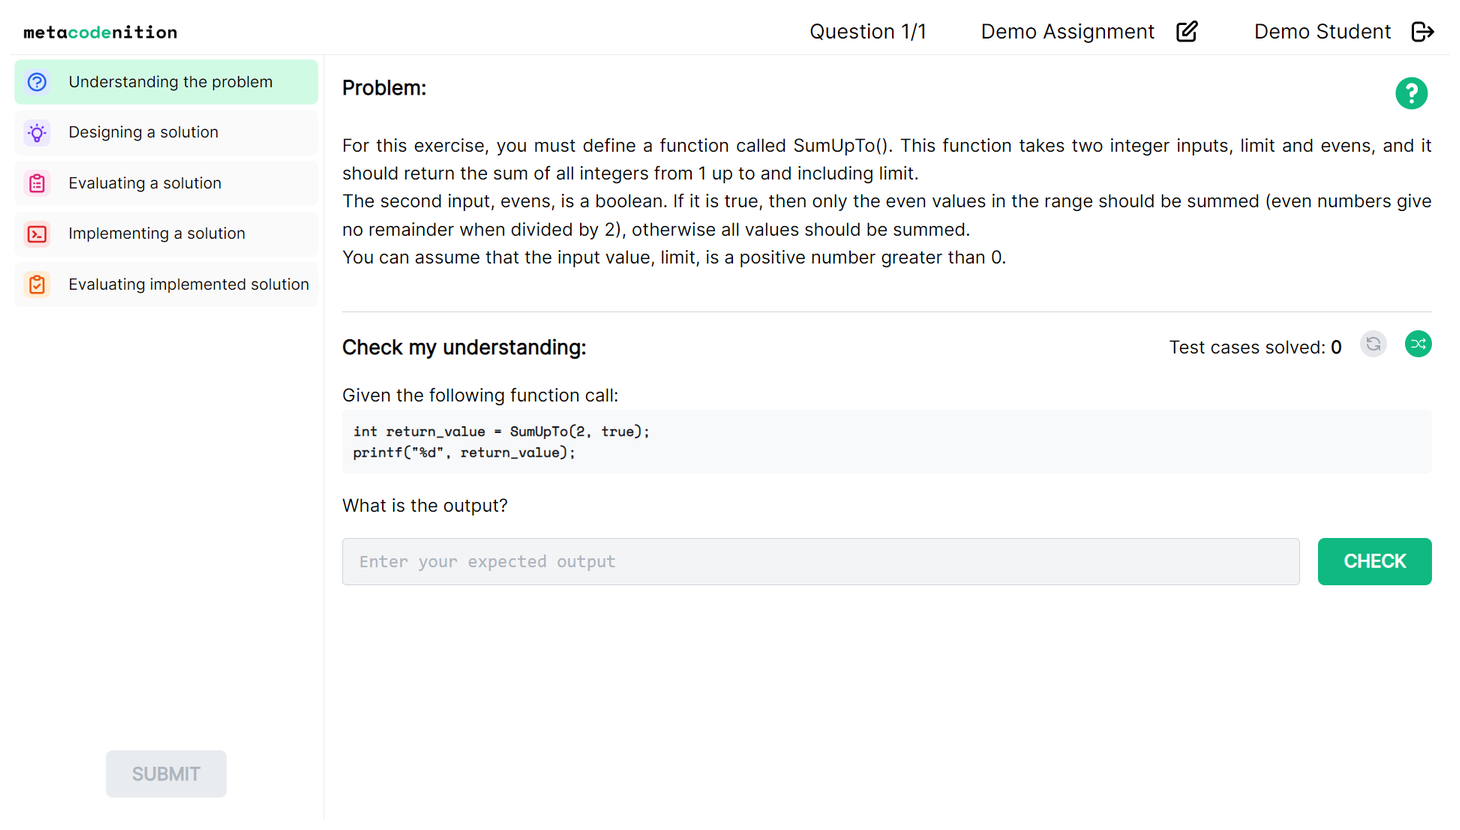
\includegraphics[width=\linewidth]{understanding-the-problem}
  \caption{Understanding the problem page.}
  \Description{A screenshot of Metacodenition's understanding the problem page.}
  \label{fig:understanding}
\end{figure}

\subsubsection{Designing a solution}
The \emph{designing a solution} stage is where a student reads through the problem and identifies programming patterns they have used or encountered in the past which may be relevant. Figure \ref{fig:designing} shows the \emph{designing a solution stage} on Metacodenition. A problem-solving tool should integrate and link the programming exercise text to the code constructs and have formatting and commenting features for the text and code \cite{saenz2022}. In Metacodenition, this is achieved by highlighting parts of the problem that the student thinks require code to achieve and assigning an action to it. By assigning an action to a part of the problem, the student identifies a programming pattern or code construct that they can use to address that part of the problem. For example, the student may identify that a modulo operator can be used to check if a value is even.

\begin{figure}[h!]
  \centering
  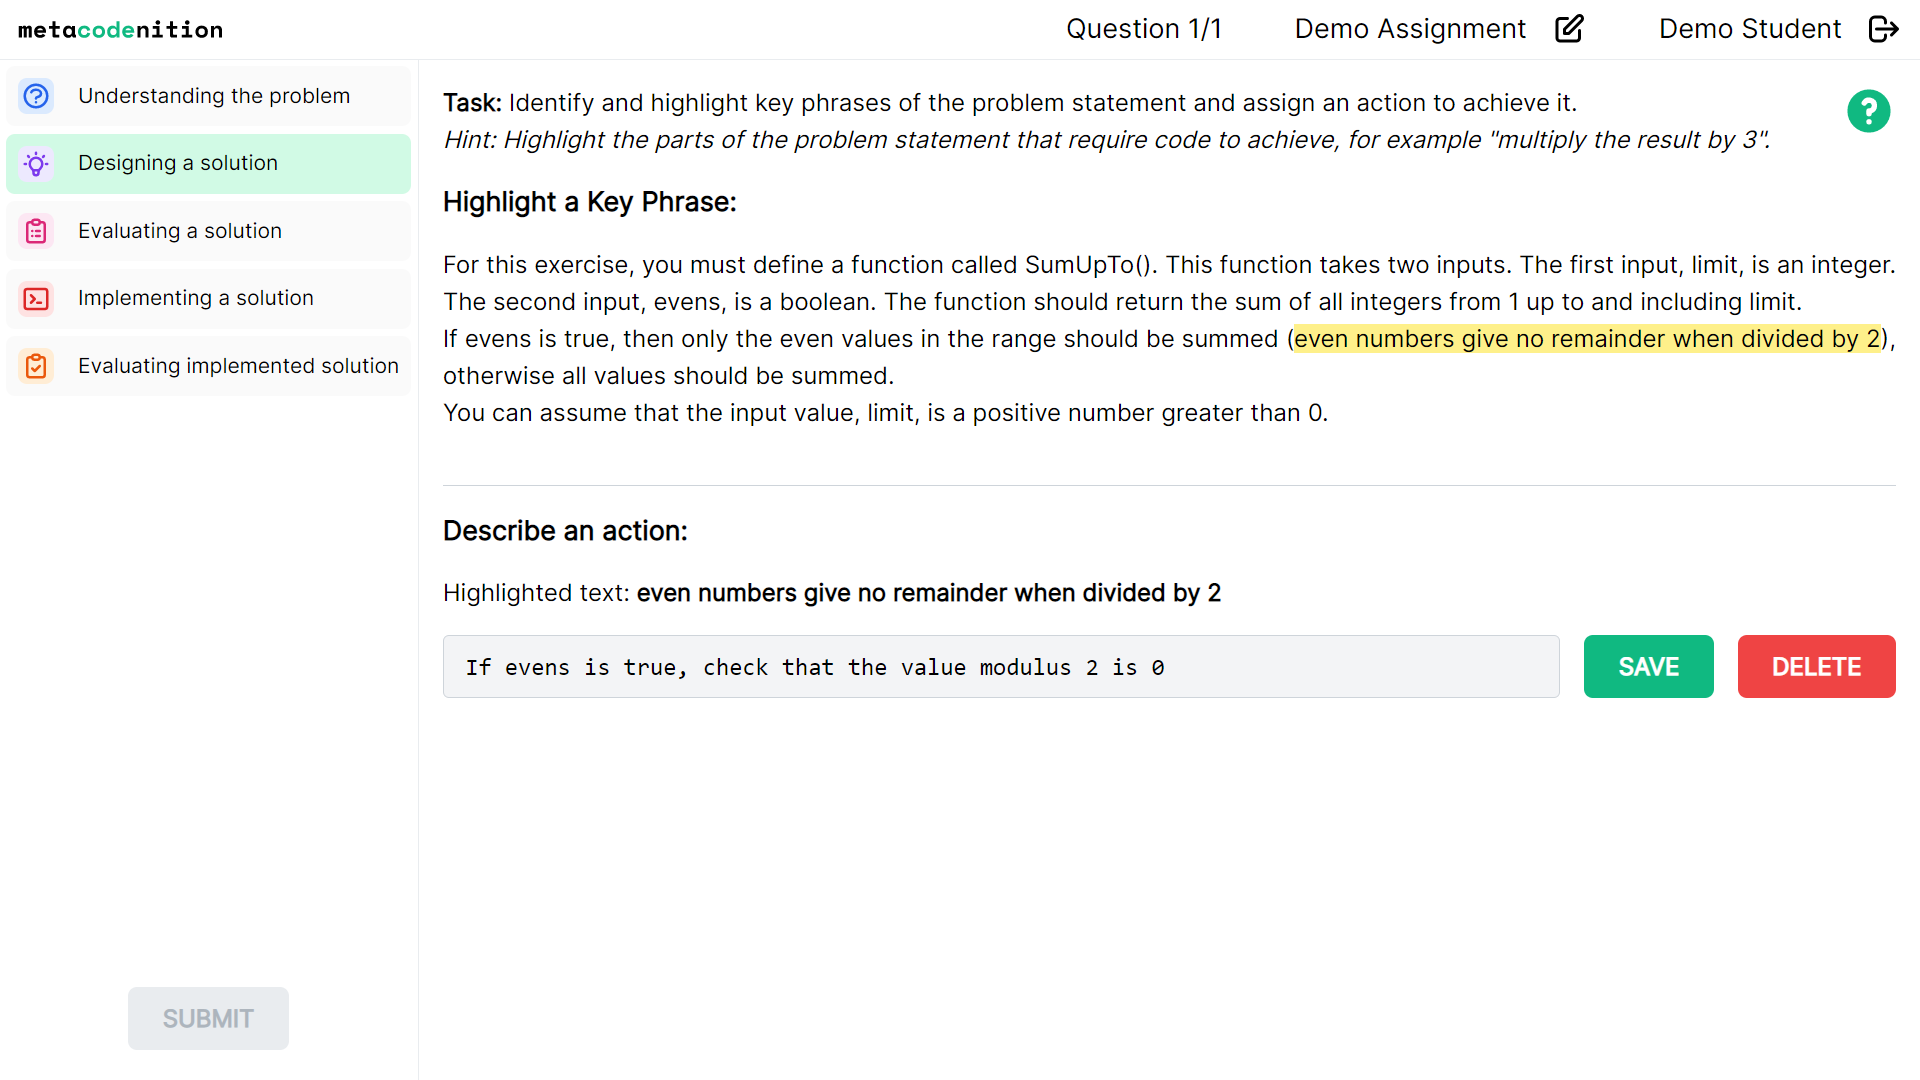
\includegraphics[width=\linewidth]{designing-a-solution}
  \caption{Designing a solution page.}
  \Description{A screenshot of Metacodenition's designing a solution page.}
  \label{fig:designing}
\end{figure}

\subsubsection{Evaluating a solution}
The \emph{evaluating a solution} stage (see Figure \ref{fig:evaluating}) is where a student forms an action plan for their program by selecting and rearranging actions they created previously in the \emph{designing a solution} stage. Students can do this by dragging and dropping blocks from the \emph{My Actions} section to the \emph{My Action Plan} section. There is also functionality to create new actions if a student feels that the actions they generated previously are insufficient. This stage is inspired by design parsons problems \cite{garcia2021}, where instead of students being provided with fragments to rearrange, students use previously created fragments. In designing Metacodenition, we particularly wanted to have good interconnection of stages to support a good flow through the problem-solving process. Using users' previously created actions, we found a more suitable solution for our goal of interconnection than pre-defined fragments.

\begin{figure}[h!]
  \centering
  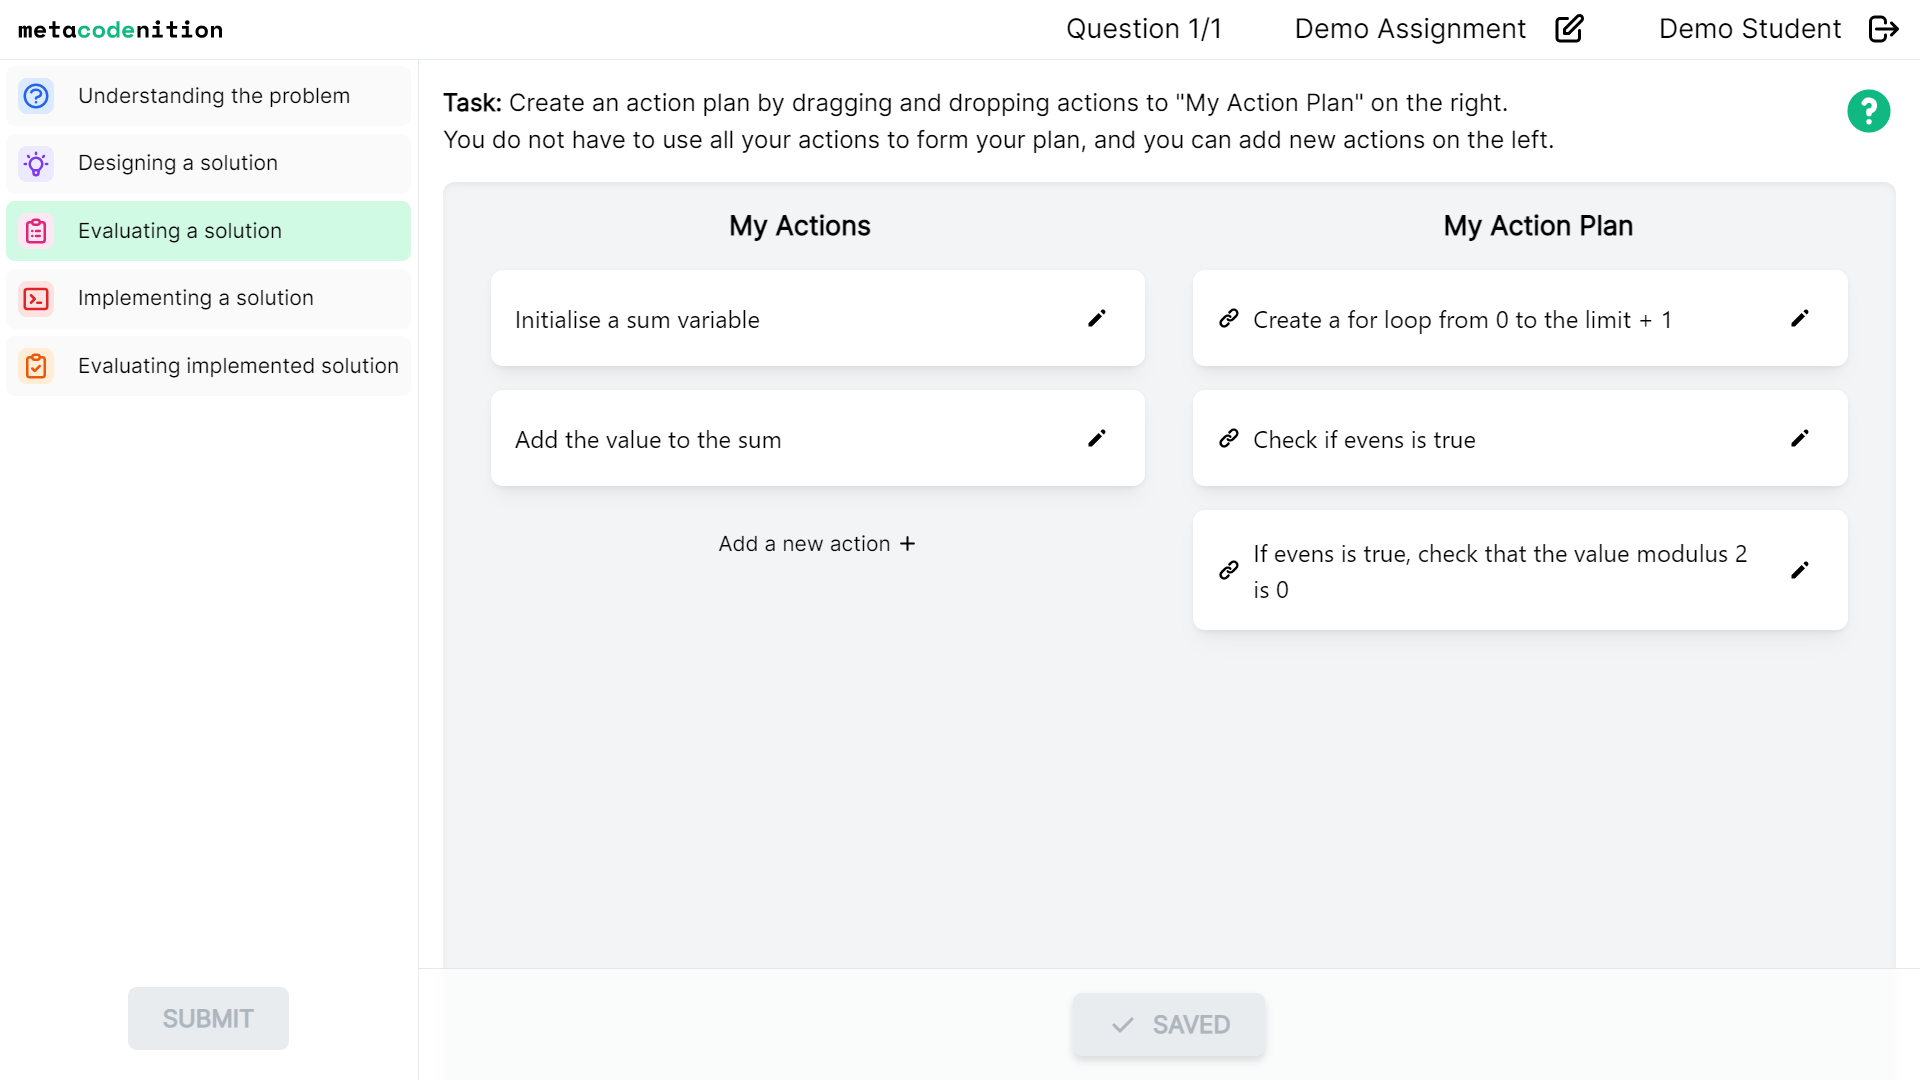
\includegraphics[width=\linewidth]{evaluating-a-solution}
  \caption{Evaluating a solution page.}
  \Description{A screenshot of Metacodenition's evaluating a solution page.}
  \label{fig:evaluating}
\end{figure}

\subsubsection{Implementing a solution}
The \emph{implementing a solution} stage is where students write their code, as shown in Figure \ref{fig:implementing}. This screen is split into two sections: an area to write their code and a panel with three different tabs. A problem-solving tool should integrate and link the programming exercise text to the code constructs \cite{saenz2022}, which we address in the page's tab design. Tab 1, the default tab, shows the previous action plan the student created, which can be used to inform their solution. Tab 2 shows the problem statement along with its highlights and assigned actions. Tab 3 is an area where students can run and debug their code.

\begin{figure}[h!]
  \centering
  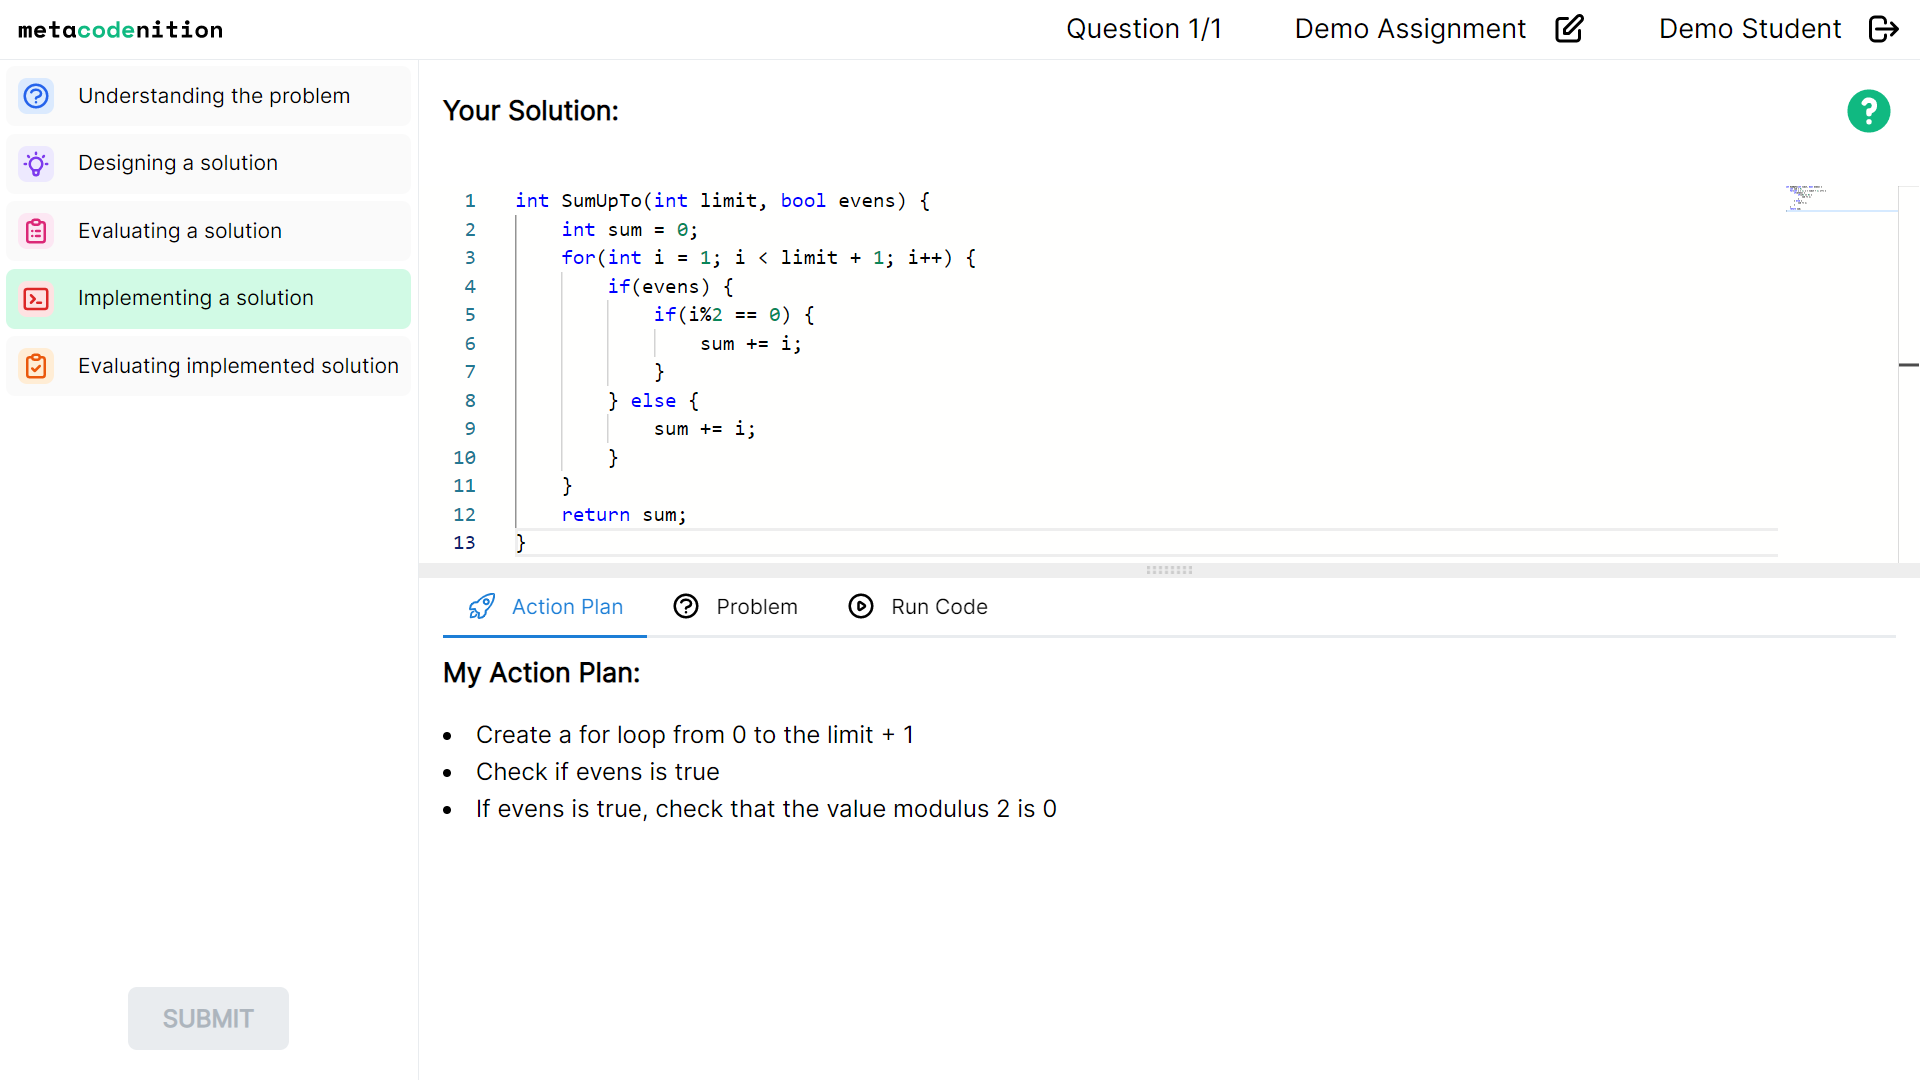
\includegraphics[width=\linewidth]{implementing-a-solution}
  \caption{Implementing a solution page.}
  \Description{A screenshot of Metacodenition's implementing a solution page.}
  \label{fig:implementing}
\end{figure}

\subsubsection{Evaluating implemented solution}
In the \emph{evaluating implemented solution} stage, students can test their code against test cases they previously solved in the \emph{understanding the problem} stage. Test cases they did not solve previously are disabled. Students also have the option to add test cases. Figure \ref{fig:evaluatingimplemented} shows the user interface for this stage \ref{fig:evaluatingimplemented}. The functionality of solving test cases before programming and then running these test cases after programming is influenced by test-driven development (TDD) \cite{janzen2008}. Like TDD, students convert requirements from the problem statement into test cases before developing and testing their solution against all test cases. The main difference is that the students' test suites are built by solving pre-defined test cases rather than writing their own. While traditional TDD for education has proven successful in isolation, Metacodenition provides multiple non-code-writing activities for students to complete. Consequently, keeping each activity short to minimise impedance becomes particularly important to keep students motivated. 

\begin{figure}[h!]
  \centering
  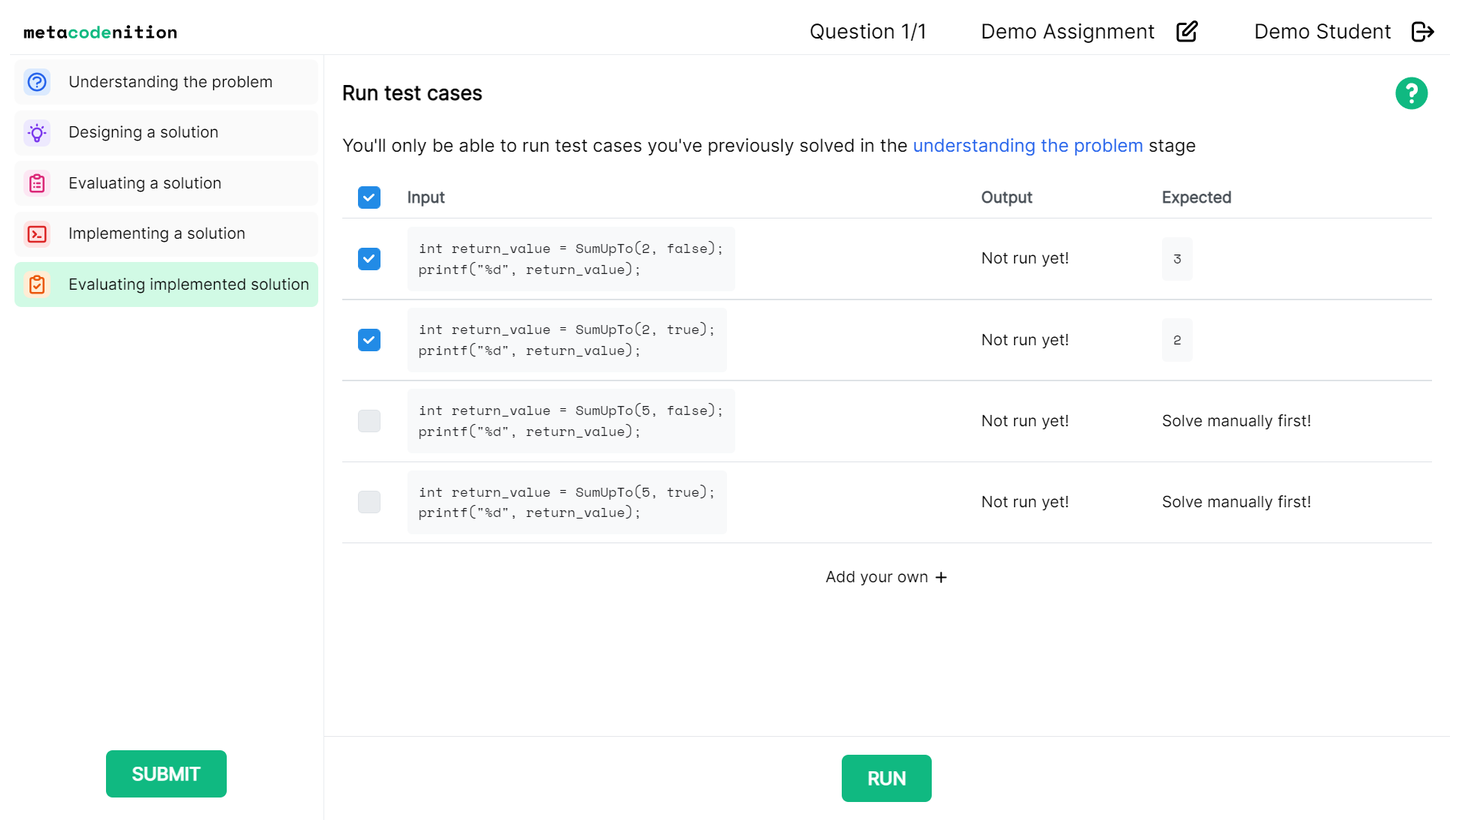
\includegraphics[width=\linewidth]{evaluating-implemented-solution}
  \caption{Evaluating implemented solution page.}
  \Description{A screenshot of Metacodenition's evaluating implemented solution page.}
  \label{fig:evaluatingimplemented}
\end{figure}

\subsection{Technologies}
Metacodenition was chosen to be developed into a web-based integrated development environment. A web based development environment is easier for students to access than a desktop application, and no configuration or installation is required. We chose to work with React.js, Mantine UI, and Tailwind CSS as the main front-end libraries, as we had familiarity with them. We selected Monaco editor as the code editor for the IDE as it is the same one used in VS Code, and offers a wide suite of functionality. For hosting our application, we chose the Firebase and Google Cloud Platform services due to their ease of use and suite of features. JobeInABox was chosen as the code-running server as this is the same server that is used to run student's code submissions in the course, and was simple to deploy to Google's Cloud Run service.

\section{Evaluation}
Metacodenition was deployed and used by 821 students in a graded lab for a first-year software engineering course at the University of Auckland. The lab had six questions about loops and arrays in the C programming language. The first three problems served as warm-up exercises to ensure that students were comfortable with functions that \emph{return} values, functions that \emph{do not return} values, and iterating through an array. These warm-up problems were provided through the regular platform used for labs, which students were instructed to solve in their own development environments. After question three, the platform asked students to solve problems four to six on Metacodenition and provided them with a link. For simplicity, we will refer to problems four to six of the lab as Metacodenition problems one to three. Table \ref{tab:problems} displays the descriptions students were provided with for each of these problems.

\begin{table}
  \caption{The problems presented on Metacodenition.}
  \label{tab:problems}
  \begin{tabular}{c|p{75mm}}
    \toprule
    \#&Problem description\\
    \midrule
    1 & Define a function called SumPositiveValues() which is passed two inputs: an array of integers, and an integer indicating how many elements are in the array. The function should return the sum of all positive integers in the input array.\\
    \midrule
    2 & Define a function called PrintSummary() which is passed one input: an array of integers of unknown length. This function should determine whether there are more positive or more negative values in the array. You should only examine values in the array until the first occurrence of the value 0. If there are more positive than negative values, you should print the word "Positive". If there are more negative values than positive values, you should print the word "Negative". If there are an equal number of positive and negative values, you should print the word "Equal".\\
    \midrule
    3 & Define a function called PrintAverageRainfall() which is passed an array of integers representing daily rainfall amounts. The function should calculate and print the average rainfall. The daily rainfall amounts are occasionally corrupted, represented by negative values, so any negative value should be ignored from your calculation. The array also contains a special value, -999, to indicate the end of the valid rainfall data, so you should only examine values in the array up to the first occurrence of the value -999. Print the average of the valid rainfall data, rounded to 2d.p. If there are no valid rainfall values then print "no rain". \\
  \bottomrule
\end{tabular}
\end{table}

\subsection{User groups}
To address our research question about the effect of scaffolding on the amount of failed test cases in final submissions, we split students into one of two user groups (A or B) when they logged in to Metacodenition. Of the 821 students who used Metacodenition, 392 were in group A, and 429 were in group B. For problem one, students in user group A were provided with all scaffolding, while students in user group B were only given the \emph{implementing a solution} stage and vice versa for problem two. Table ~\ref{tab:scaffoldingConfig} summarises this configuration. When students got to problem three, they were prompted to select which problem-solving stages they would like to use. This setup was designed to ensure all students had a fair chance to try all interventions while still allowing us to answer our research question. Final submissions for all problems were recorded. We hypothesise that submissions from the user group who received all scaffolding will have a smaller percentage of test cases that failed for each question.

\begin{table}
  \caption{Summary of the configuration of the scaffolding made available to each user group for each problem.}
  \label{tab:scaffoldingConfig}
  \begin{tabular}{c|p{30mm}|p{30mm}}
    \toprule
   Problem \#&Group A&Group B \\
    \midrule
    1&All scaffolding&Only \emph{implementing a solution} \\
    \midrule
    2&Only\emph{implementing a solution}&All scaffolding \\
    \midrule
    3&Choice of scaffolding&Choice of scaffolding \\
    \bottomrule
  \end{tabular}
\end{table}

\subsection{Questionnaire}
At the end of the lab, an optional questionnaire was displayed for students to answer. The following questions were asked to address our research question of student perceptions of Metacodenition:
\begin{enumerate}
    \item How helpful was the problem-solving assistance?
    \item Which assistance was the most helpful?
    \item I would use this tool again if it was optional (True or False).
    \item What worked well?
\end{enumerate}
Question one was a five-point scale question which asked students to rank how easy it was to use Metacodenition from zero (extremely difficult) to five (extremely easy). Question two was close-ended, allowing students to select a problem-solving stage. Question three was a close-ended question presented as a checkbox, allowing students to check if they agreed with the statement. Question four was an open-ended question intended to collect student anecdotes.

The questionnaire also included a number of questions to identify room for improvement or any bugs that students encountered:
\begin{itemize}
    \item How easy was it to use this tool?
    \item What went wrong?
\end{itemize}

\section{Results and Discussion}
\subsection{Test cases failed in final submissions}
The metric we used to measure a user group's performance was the percentage of test cases that a user group's final submissions failed. A final submission refers to the source code that a student submits to Metacodenition (only one submission is allowed per student). We ran all final submissions against the test suite, which consists of the test cases available to students in the \emph{evaluating implemented solution} stage and additional "hidden" test cases covering edge cases. Tables 3 and 4 present the test suites we run final submissions against and the count of submissions which failed each test case per user group. Table 3 presents the test suite for problem 1, while Table 4 presents the test suite for problem 2.

\begin{table*}
  \caption{Test cases failed in final submissions for problem one.}
  \label{tab:freq}
  \begin{tabular}{l|c|c|c|c|c}
    \toprule
    \multirow{2}{*}{Input Array} & \multirow{2}{*}{Input Length} & \multirow{2}{*}{Expected Output} & \multirow{2}{*}{Hidden (Y/N)} & \multicolumn{2}{c}{Failed Count} \\
    \cmidrule{5-6}
    & & & & A & B \\
    \midrule
    \{1, 2, 3\} & 0 & 0 & N & 7 & 20 \\
    \midrule
     \{1, 2, 3\} & 2 & 3 & N & 7 & 25 \\
    \midrule
    \{1, 2, 3\} & 3 & 6 & N & 8 & 23 \\
    \midrule
    \{-5, -4, -3, -2, -1, 0, 1, 2, 3, 4, 5\} & 6 & 0 & N & 9 & 124\\
    \midrule
    \{-5, -4, -3, -2, -1, 0, 1, 2, 3, 4, 5\} & 11 & 15 & N & 9 & 125\\
    \midrule
    \{-150, 150\} & 2 & 150 & N & 10 & 124\\
    \midrule
    \{125, 125, -256, 328\} & 4 & 578 & Y & 11 & 125\\
    \midrule
    \{10000, 30000, -100000\} & 3 & 4000 & Y & 11 & 124\\
    \midrule
    \{-250000, -100000, -14, 3\} & 4 & 3 & Y & 10 & 125 \\
    \midrule
    \{1024, 1024, 2048, 4096, -8192\} & 5 & 8192 & Y & 11 & 125\\
    \midrule
    \{1, 2, 3, 0\} & 0 & 0 & Y & 7 & 20 \\
  \bottomrule
\end{tabular}
\end{table*}

\begin{table*}
  \caption{Test cases failed in final submissions for problem two.}
  \label{tab:freq}
  \begin{tabular}{l|c|c|c|c|c}
    \toprule
    \multirow{2}{*}{Input Array} & \multirow{2}{*}{Expected Output} & \multirow{2}{*}{Hidden (Y/N)} & \multicolumn{2}{c}{Failed Count} \\
    \cmidrule{4-5}
    & & & A & B \\
    \midrule
    \{1, 2, 3, 0\} & Positive & N & 46 & 32 \\
    \midrule
     \{0, 1, 2, 3\} & Equal & N & 46 & 34 \\
    \midrule
    \{-1, 0, 1, 2, 3\} & Negative & N & 49 & 34 \\
    \midrule
    \{-5, -4, -3, -2, -1, 0, 1, 2, 3, 4, 5\} & Negative & N & 47 & 33\\
    \midrule
    \{-5, -4, -3, -2, -1, 1, 2, 3, 4, 5, 0\}& Equal & N & 50 & 34\\
    \midrule
    \{-150, 15, 10, 0\}& Positive & N & 50 & 37\\
    \midrule
    \{1000000000, -1, -1, 0\}& Negative & Y & 52 & 32\\
    \midrule
    \{1, -1, 1, -1, 1, -1, 1, -1, 0, 1, -1, 1\}& Equal & Y & 50 & 36\\
    \midrule
    \{1, -1, 1, -1, 1, -1, 1, -1, 1, 0, -1, 1\}& Positive & Y & 50 & 37 \\
    \midrule
    \{1, -1, 1, -1, 1, -1, 1, -1, -1, 0, 1, 1\}& Negative & Y & 51  & 35\\
    \midrule
    \{0\}& Equal & Y & 46 & 33 \\
    \midrule
    \{-4123, -58182, -16, 3, 1, 7, 8, 0\}& Positive & Y & 53 & 36 \\
  \bottomrule
\end{tabular}
\end{table*}

Figure \ref{fig:testcases} shows a bar graph of the percentage of test cases that failed in final submissions per user group per problem. We see that for problem 1, the percentage of test cases failed by group A, which received scaffolding for this problem, is approximately 2\%, compared to approximately 22\% by group B. For problem 2, the percentage of test cases failed by group B is approximately 8\%, in contrast to approximately 13\% by group A. These results show that students who receive all scaffolding tend to fail fewer test cases than students who receive no scaffolding. This result could be attributed to students who received all interventions having the ability to view the test suite (understanding the problem) and test their code against it  (evaluating implemented solution) before submission. However, as we see in Tables 3 and 4, this trend still holds for hidden test cases, which neither students with scaffolding nor without could view or test their code against. Additionally, students could still manually run test cases when they did not have scaffolding. The difference is that when students had scaffolding, they were explicitly prompted to run their code against test cases. When they did not have scaffolding, they were not made aware of their problem-solving state or the corresponding actions to take. We believe this indicates that Metacodenition's scaffolding positively affects test case failure rates. We also see that the gap between the percentage of failed test cases is smaller for problem two than for problem one. A possible explanation is that the group of students who did not receive scaffolding for problem two had previously received scaffolding for problem one and had become more metacognitively aware. Hence, they self-initiated the task of running test cases.

\begin{figure}[h!]
  \centering
  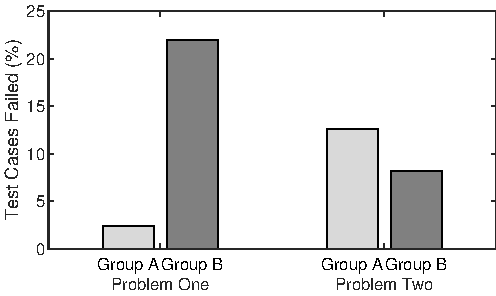
\includegraphics[width=\columnwidth]{test_cases}
  \caption{Percentage of test cases failed for final submissions per user group per question.}
  \Description{A bar graph showing the percentage of test cases failed in final submissions per user group per question.}
  \label{fig:testcases}
\end{figure}

\subsection{Student perceptions of Metacodenition's scaffolding}
Most students found the scaffolding provided by the \emph{evaluating implemented solution} stage the most helpful. The second most helpful stage deemed by students was the \emph{understanding the problem} stage. Figure \ref{fig:interventions} presents a bar graph of the number of students who indicated each stage to be the most helpful. It is no surprise that students found \emph{evaluating implemented solution} to be the most helpful, as this stage appears to contribute the most to the final solution. The popularity of \emph{understanding the problem} is also expected, as this intervention is backed up by past studies showing positive results. Still, it is good to see that this stage was well received by students when combined with the other scaffolding in Metacodenition, as past work studied it in isolation.

\begin{figure}[h!]
  \centering
  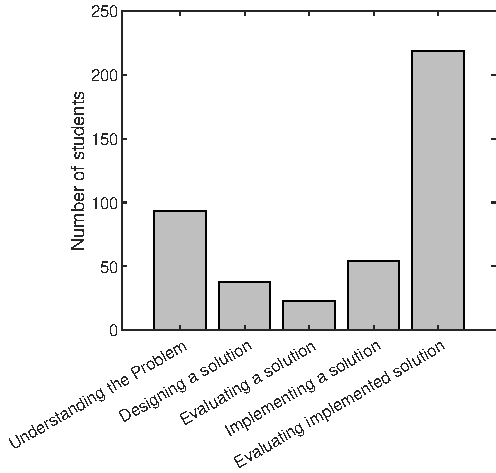
\includegraphics[width=\columnwidth]{intervention_responses}
  \caption{Responses to "Which assistance was the most helpful?".}
  \Description{A bar graph showing responses to the "Which assistance was the most helpful?" in the questionnaire.}
  \label{fig:interventions}
\end{figure}

Figure \ref{fig:usefulness} shows a histogram of student responses to "How helpful was the problem-solving assistance?". We see that the mean rating is approximately 3.18 out of 5, which corresponds to "helpful". Of the 427 students who answered the questionnaire, 304 student agreed with the statement "I would use this tool again if it was optional". Together, these results indicate that most students perceived Metacodenition as a helpful tool they would use again, even if not required.

\begin{figure}[h!]
  \centering
  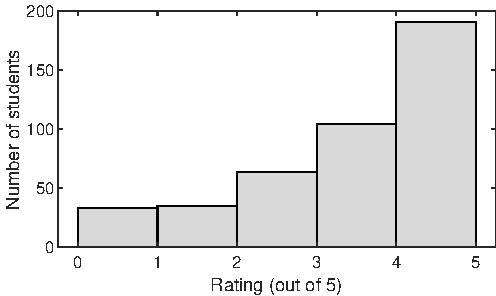
\includegraphics[width=\columnwidth]{usefulness_responses}
  \caption{Responses to "How helpful was the problem-solving assistance?".}
  \Description{A bar graph showing responses to the "Which assistance was the most helpful?" in the questionnaire.}
  \label{fig:usefulness}
\end{figure}

In the open-ended responses for "What worked well?", many students expressed that they liked a certain stage of Metacodeniton:
\begin{itemize}
    \item "Understanding the problem was a huge help. Not only did it allow for easy testing later but often there is a bit of ambiguity of what to do in a specific case so its really nice to have that sorted before I started coding."
    \item "I liked the Test cases and the highlighting of the question sections. I found I fully understood all the edge cases and sentences in the question that I would typically miss."
     \item "Requiring the user to highlight and explain parts of the brief makes it much easier to make a pseudo code."
     \item "It was exactly like writing a pseudocode, except you could change the order of your plan easily. It was just super helpful to type down notes and clear my head before I started coding."
    \item "I really liked how I could write out a solution plan which outlined what I needed to do, and how it remained visible as I was writing my code."
    \item "I found the evaluating part helpful as it allowed me to see all the tests together and see patterns in the tests that failed."
\end{itemize}

Other students indicated that they particularly liked how the \emph{understanding a problem} and \emph{evaluating implemented solution} stages linked together:
\begin{itemize}
    \item "It was good to be able to manually solve the expected outputs and then test my code on those same test cases."
    \item "I like how we are able to check our code solution to something we hand worked first."
    \item "Manually working out answers and then comparing them to the code's actions was very useful."
\end{itemize}

Multiple students expressed interest in enhanced compiler error messages (ECEMs), with one stating: "Some of the error messages are vague or hard to understand to inexperienced coders". Multiple students indicated an interest in a specific ECEM, which is being informed when their code enters an infinite loop:
\begin{itemize}
    \item "If a while loop prints something infinitely, it makes the output text box stretch out."
    \item "Occasionally when my code didn't work, it didn't produce any output or give any error message so it was hard to move further."
\end{itemize}

Interestingly, one student responded, "Felt like learning a new skill" to the question on what went wrong. Though this student felt that this went wrong, we consider their response to be a positive indicator that Metacodenition achieved what we intended it to do - which is to teach students problem-solving skills.

\subsection{Limitations}
One limitation is that our evaluation was conducted with a limited scope, taking place in a single lab over a week. Problem-solving skills take time to develop, so a longer time frame is needed to evaluate Metacodenition's interventions accurately. Future studies should investigate Metacodenition's benefits over a more extended period, such as over a semester.

Another potential limitation could have been introduced by some students knowing this study was conducted by fourth-year engineering students for a part four project. These students could have had a courtesy bias, preventing them from giving negative feedback in our questionnaire.

Additionally, a limitation of our evaluation could have stemmed from the bugs reported by students, which were fixed during the first two days. Students who accessed the tool on different days may have had different experiences. These students likely had a cognitive bias where the bugs they experienced were heavily weighted in their overall judgement of Metacodenition, resulting in more negative feedback (peak-end rule).

\section{Conclusions}
This paper presented our approach to designing and evaluating a tool for novice programmers called Metacodenition, which provides metacognitive scaffolding for a problem-solving framework. By scaffolding the problem-solving process from start to finish, Metacodention aims to promote the development of problem-solving skills in novices. Results from our evaluation show fewer test cases failed in the final submissions of students who received all of Metacodenition's scaffolding compared to students who received only the \emph{implementing a solution} stage. We also found that most students perceived Metacodenition as a helpful tool they would voluntarily use in the future. 

Student feedback has highlighted a potential direction for improving Metacodenition, specifically in adding enhanced compiler error messages. Loksa et al.'s problem-solving framework also included the \emph{searching for analogous problems} stage that Metacodenition omitted. Here, students draw upon problems they have encountered previously. Additional future work could include adding an intervention for this stage to Metacodenition. We suggest a "problem bank" of past problems a student has solved and their corresponding solutions, allowing them to identify and filter relevant problems (ones with similar patterns).

\bibliographystyle{ACM-Reference-Format}
\bibliography{refs}

\end{document}
\endinput
%%
%% End of file `main.tex'.
